\documentclass[areasetadvanced]{scrartcl}

\usepackage[utf8]{inputenc}
\usepackage[T2A]{fontenc}
\usepackage[english,russian]{babel}

\usepackage[footskip=1cm,left=25mm, right=15mm, top=20mm, bottom=20mm]{geometry}
\usepackage{setspace}
\usepackage{amsmath, amssymb}  % Объединено в одну строку
\usepackage{graphicx}
\usepackage{tikz}
\usetikzlibrary{arrows.meta}
\usepackage{float}
\usepackage{dashrule}
\usepackage{fancyhdr} % оформление отчёта
\usepackage{hyperref} % оформление отчёта
\usepackage{textcomp, enumitem}
\usepackage{indentfirst}
\usepackage{graphicx}
\setlength{\parindent}{1.25cm}
\usepackage{algorithm}
\usepackage{algpseudocode}
\usepackage{array}  % Для использования команды m{}
\usepackage{geometry}
\usepackage{afterpage}
\usepackage{minted}
\setcounter{secnumdepth}{3}  % Включает нумерацию для subsubsection
\setcounter{tocdepth}{3}     % Включает subsubsection в содержание
\usepackage{listings} % Если используете listings

\tikzstyle{block} = [rectangle, rounded corners, minimum width=3cm, minimum height=1cm, text centered, draw=black, fill=lightgray]

\setkomafont{sectioning}{\normalfont\bfseries} % для заголовков разделов и подразделов
\setkomafont{section}{\normalfont\Large\bfseries}
\setkomafont{subsection}{\normalfont\large\bfseries}
\setkomafont{subsubsection}{\normalfont\large\bfseries}
\setkomafont{paragraph}{\normalfont\large\bfseries} % для заголовков параграфов (если они есть)

\lstset{
  language=Haskell,
  basicstyle=\ttfamily\small,
  keywordstyle=\color{blue}\bfseries,
  stringstyle=\color{red},
  commentstyle=\color{green!70!black},
  numbers=left,
  numberstyle=\tiny,
  stepnumber=1,
  numbersep=10pt,
  showstringspaces=false,
  breaklines=true,
  frame=single
}

\setcounter{tocdepth}{2}
\begin{document}
\setlength{\parindent}{1.25cm}
\setlength{\parskip}{\baselineskip}
	\thispagestyle{empty}
	\begin{center}
		\large{МИНОБРНАУКИ РОССИИ} \par
		\vspace{0.3cm}
		\normalsize
		{ФЕДЕРАЛЬНОЕ ГОСУДАРСТВЕННОЕ АВТОНОМНОЕ ОБРАЗОВАТЕЛЬНОЕ УЧРЕЖДЕНИЕ ВЫСШЕГО ОБРАЗОВАНИЯ} \par
		\vspace{0.3cm}
		\textbf{\guillemotleft САНКТ-ПЕТЕРБУРГСКИЙ ПОЛИТЕХНИЧЕСКИЙ}
		\textbf{УНИВЕРСИТЕТ ПЕТРА ВЕЛИКОГО\guillemotright} \par
		\vspace{0.3cm}
		{Институт компьютерных наук и кибербезопасности}\par
		{Высшая школа технологий искусственного интеллекта}\par
	\end{center}
	\vfill
	\begin{center}
		{\large Доклад по дисциплине \guillemotleft Методы тестирования ПО\guillemotright}\par
		{\huge  Основные задачи технологии тестирования Фаззинг }
         
	\end{center}
	\vfill
	\begin{flushleft}
		Студент: \hspace{1.8cm} \rule[0pt]{2.5cm}{0.5pt}\hfill Салимли Айзек Мухтар Оглы\par
		\vspace{1.5cm}
		Преподаватель: \hspace{0.55cm} \rule[0pt]{2.5cm}{0.5pt}\hfill  Курочкин Михаил Александрович
	\end{flushleft}
	\vspace{0.5cm}
	\begin{flushright}
		\guillemotleft \rule[0pt]{0.8cm}{0.5pt}\guillemotright \rule[0pt]{2cm}{0.5pt} 20\rule[0pt]{0.5cm}{0.5pt} г.
	\end{flushright}
	\vfill
	\begin{center}
		Санкт-Петербург, 2025
	\end{center}
	\newpage
	\tableofcontents
	\newpage
\section*{Введение}
	\addcontentsline{toc}{section}{Введение}
    В данном докладе рассматривается применение технологии фаззинг (Fuzzing) для тестирования
    программного обеспечения на наличие уязвимостей, когда вместо ожидаемых входных данных
    программе передаются случайные или специально сформированные данные.
    Рассмотрены основные типы, этапы фаззинга и их эффективность, что такое метод серого ящика и
    зачем для фаззинга нужны санитайзеры.
\newpage
\section{Фаззинг}
Фаззинг — техника тестирования программного обеспечения, часто автоматическая или
полуавтоматическая, заключающаяся в передаче приложению на вход неправильных,
неожиданных или случайных данных. Предметом интереса являются падения и зависания,
нарушения внутренней логики и проверок в коде приложения, утечки памяти, вызванные такими
данными на входе. Фаззинг является разновидностью выборочного тестирования (англ. random
testing), часто используемого для проверки проблем безопасности в программном обеспечении и
компьютерных системах. В качестве входных данных при этом могут выступать обрабатываемые
приложением файлы, информация, передающаяся по сетевым протоколам, функции прикладного
интерфейса и т. д.
\newpage
\section{Этапы фаззинга}
В основном этапы фаззинга состоят из:
\begin{enumerate}
    \item Анализ исследуемого приложения
    \item Разработка фаззера (опционально)
    \item Генерация данных
    \item Сам, фаззинг
    \item Анализ результатов
\end{enumerate}
\newpage
\section{Метод серого ящика}
На стыке методов структурного и функционального тестирования находится метод «серого
ящика». При тестировании данным методом исследователь не имеет полной спецификации
программы и исходных кодов, как это бывает при тестировании методом «белого ящика», однако
знаний о системе больше чем при тестировании методом «черного ящика».
Фаззинг берет лучшее от двух существующих подходов. Мы не ограничиваем себя конечным
количеством тестовых случаев и постоянно генерируем случайные входные данные для нашего
кода, но при этом каждая новая последовательность использует информацию из предыдущих
попыток для максимизации результата.
Сразу возникает резонный вопрос — могут ли случайные данные что-то протестировать в
действительности? Предположим, мы хотим проверить компилятор С/C++ и посылаем на вход
сгенерированные последовательности символов. Совершенно очевидно, что мы получим много
ошибок от компилятора на стадии лексикографического анализа и парсера выражений, но при
этом едва затронем оптимизацию и генерацию кода.
\begin{figure}[H]
    \begin{center}
      \centering
      
\includegraphics[width=0.7\textwidth]{image.png}
      \caption{Серый ящик.}
      \label{fig:syntdiag}
    \end{center}
  \end{figure}

\newpage
\section{Санитайзеры}
Санитайзеры – это инструменты для динамического тестирования, помогающие в поиске самых
разных ошибок в программах.
Повод для использования санитайзеров: переполнение буферов (глобальных, на стеке или в куче),
использование после освобождения, утечки памяти, обращение к неинициализированным
переменным.
Они также позволяют обнаруживать состояние гонки для потоков, ситуации взаимной
блокировки, обращения по нулевому указателю, деление на ноль (куда же без него),
переполнения для типов данных и некорректные битовые сдвиги.
Санитайзеры очень помогают во время отладки. Для их использования достаточно
скомпилировать исходники с включенной инструментацией, которая добавит специальные
команды в исполняемый файл. По ним можно будет следить за ходом выполнения программы и
состоянием памяти. При обнаружении ошибок будет сгенерирован отладочный вывод и
программа завершит работу.
Таким образом, мало просто сгенерировать фаззером некорректные входные данные, которые
обрушат программу. Ошибку следует устранить, а для этого надо собрать максимум информации.
Именно в этом и помогают санитайзеры. Их совместное использование повышает эффективность
тестирования.
\newpage
\section{Типы фаззеров}
Существует несколько основных типов фаззеров, они отличаются подходами к генерации входных
данных. Некоторым для работы требуется стартовый набор примеров, другим нужны правила, по
которым эти примеры могут быть выведены. Важную роль также играет случайность, которая
позволяет фаззерам создавать новые входные данные.
\subsection{На основе грамматики}
Таким фаззерам для работы требуется определенный набор правил — грамматика для
построения входных данных. Как только фаззеру будут известны эти правила, он сможет
генерировать новые комбинации на их основе. При этом можно позволить себе иногда
отклоняться от грамматики и не всегда следовать ей, подавая на вход тестируемой программы
некорректные данные.
Подобные фаззеры генерируют хорошие, достоверные последовательности, доля случайности в
них относительно невелика. Однако важно понимать, что писать такие фаззеры — дело
трудоемкое. Во-первых, грамматику следует определить самостоятельно (в редких случаях можно
взять уже готовую). Во-вторых, качество работы фаззера будет напрямую зависеть от той
грамматики, что ему передали.
\newpage
\subsection{На основе мутаций}
Такой тип фаззеров на каждом этапе случайным образом изменяет входные данные из
предыдущих попыток. При этом для старта ему требуется набор репрезентативных входов
(корпус), который будет использоваться для дальнейших мутаций. В качестве корпуса можно взять
данные пользователей или существующие тесты. Во время своей работы такой фаззер слегка
изменяет готовые последовательности (переставляя биты и байты), комбинирует и сочетает их
вариации и подает в программу.
При этом никаких дополнительных усилий от разработчика тут не требуется (разве что написание
специальных алгоритмов мутаций), но и качество входных данных у таких фаззеров обычно
среднее.
\newpage
\subsection{На основе покрытия кода}
Подобные фаззеры устроены по принципу генетического алгоритма и стремятся максимизировать
покрытие тестового кода. С практической точки зрения это один из самых эффективных на сегодня
типов фаззеров. На этой основе работает libFuzzer.
LibFuzzer - это внутрипроцессный механизм фаззинга, управляемый охватом.
LibFuzzer связан с тестируемой библиотекой и передает нечеткие входные данные в библиотеку
через определенную точку входа фаззинга (также известную как «целевая функция»); Затем
фаззер отслеживает, какие области кода достигаются, и генерирует мутации в корпусе входных
данных, чтобы максимизировать покрытие кода.
\begin{figure}[H]
    \begin{center}
      \centering
      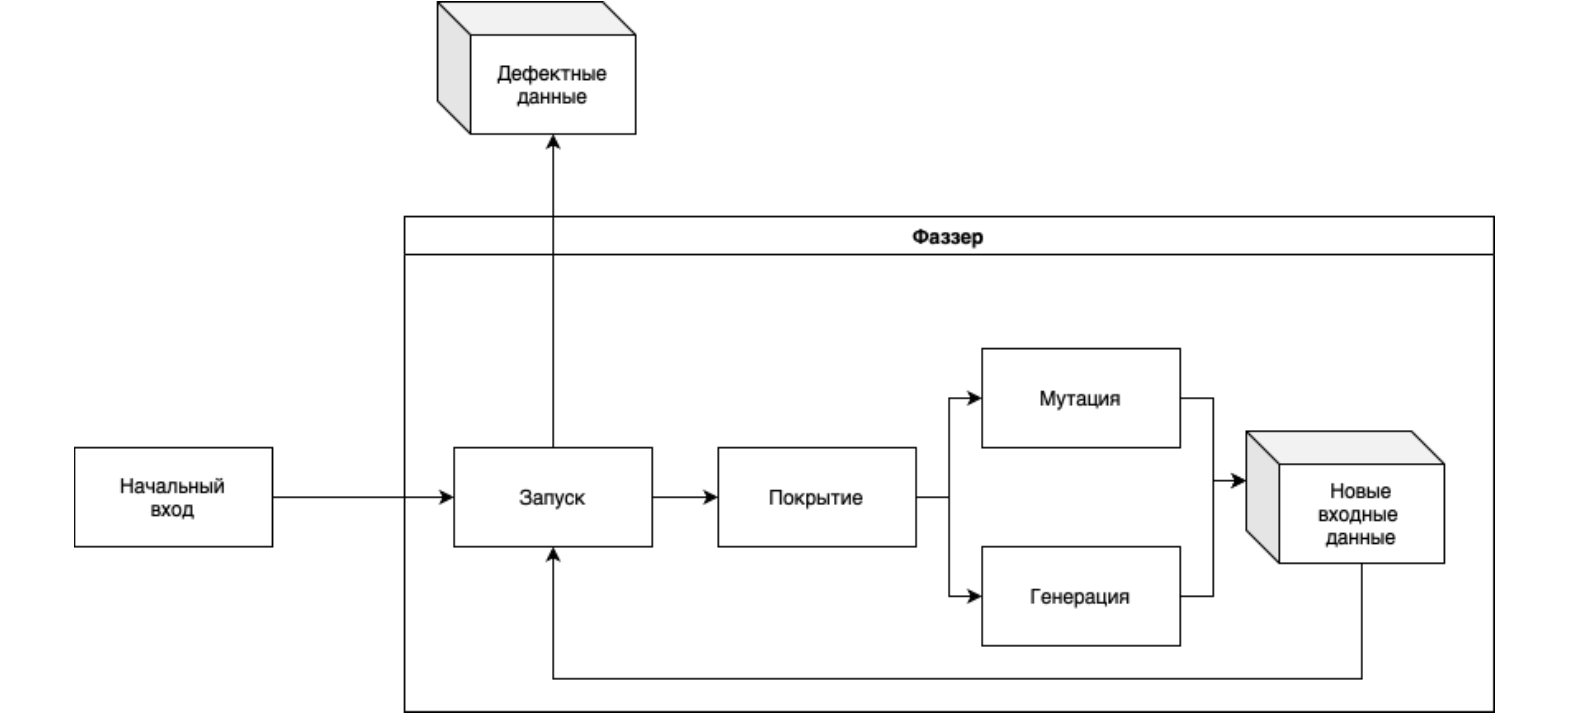
\includegraphics[width=0.7\textwidth]{image copy.png}
      \caption{Схема фаззера на основе покрытия кода.}
      \label{fig:syntdiag}
    \end{center}
  \end{figure}
\newpage
\subsection{Построение грамматики по данным}
Также есть способ сочетать подходы на основе мутаций и на основе грамматики. Специалисты по
обработке данных и машинному обучению могут попытаться построить грамматику на основе уже
имеющейся информации. Однако оценить результат на выходе таких фаззеров зачастую непросто.
\begin{figure}[H]
    \begin{center}
      \centering
      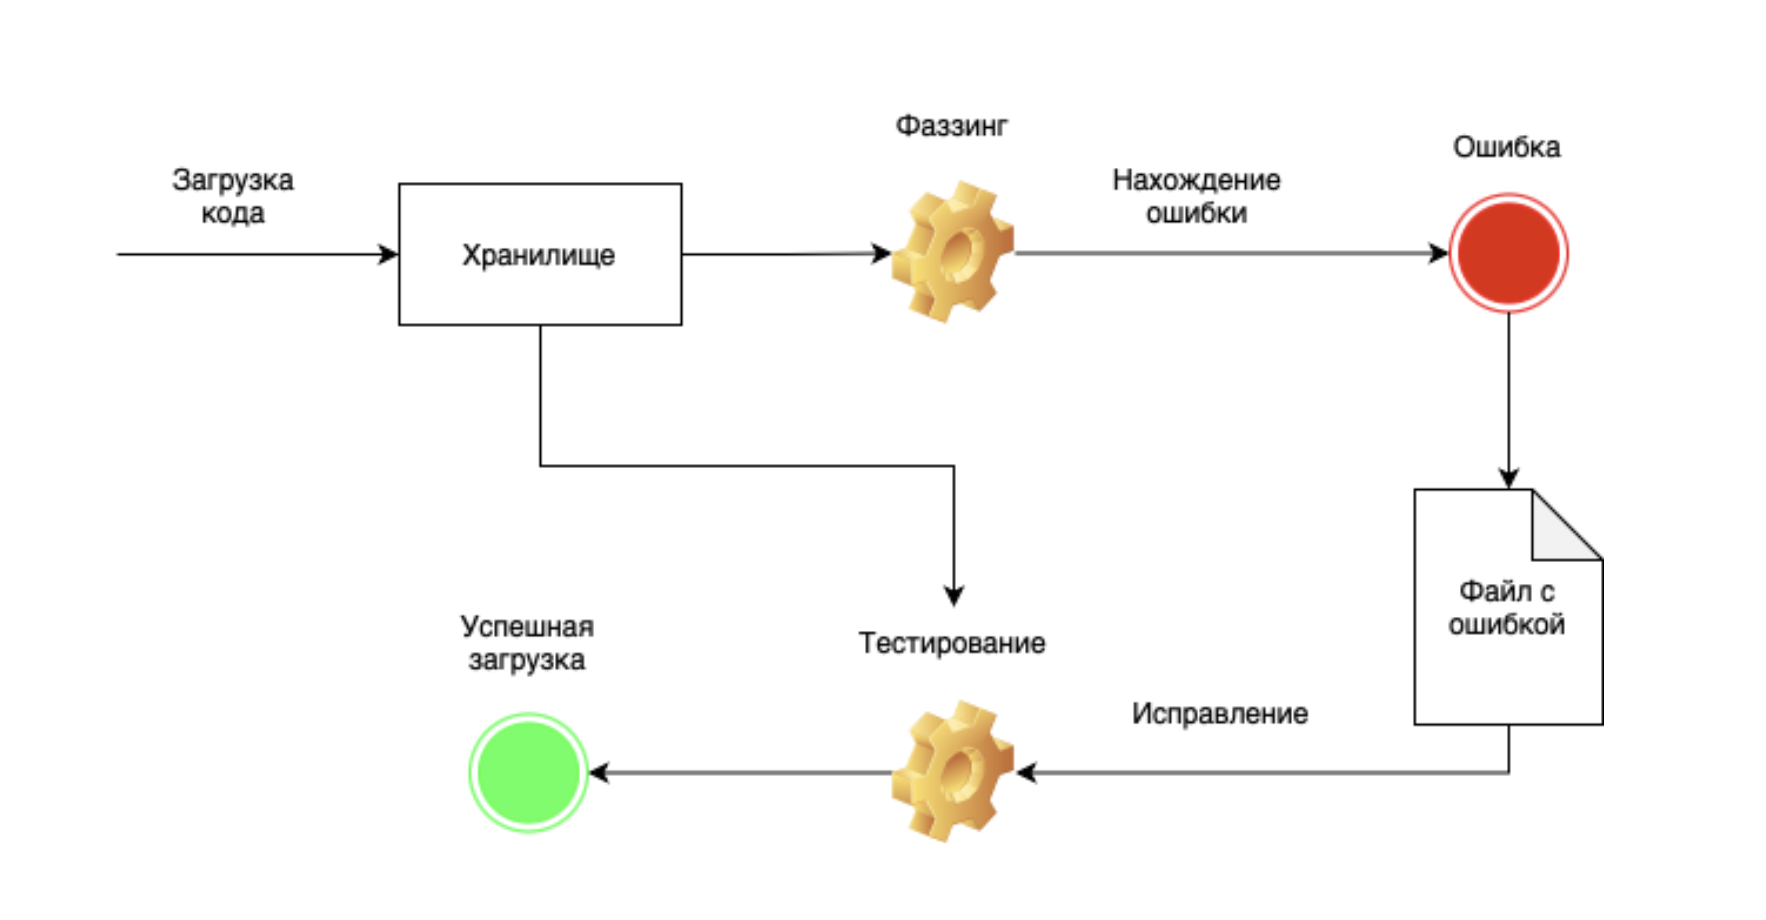
\includegraphics[width=0.7\textwidth]{image copy 2.png}
      \caption{Схема построения грамматики по данным.}
      \label{fig:syntdiag}
    \end{center}
  \end{figure}
\newpage
\section{Проблемы фаззинга}
Основные проблемы фаззинга:
\begin{itemize}
    \item Уязвимости в архитектуре
    \subitem Сложно предугадать, где найдёшь следующую уязвимость
    \item В результате фаззинга не всегда происходит падение
    \subitem Особенно при pool corruption
    \item Не все найденные уязвимости эксплуатабельны
    \subitem Таких воспроизводимых падений может быть очень много.
\end{itemize}

"Pool corruption" - ситуация когда обнаруживается повреждение или неправильное управление
памятью, связанное с выделением и освобождением памяти в программных приложениях.
Это может произойти, когда программа неправильно управляет памятью, что приводит к
потенциальной уязвимости или сбоям в работе программы.
\newpage
\section*{Заключение}
\addcontentsline{toc}{section}{Заключение}
Обнаружение даже одной уязвимости в популярном приложении за короткий срок в
автоматическом режиме может сильно помочь для тестирования и выявления критических
ошибок. Долгое время считалось, что фаззинг является слишком тяжеловесным подходом к
обнаружению программных дефектов, и полученные результаты не оправдывают затраченных
усилий и ресурсов. Однако, современные тенденции развития индустрии производства
программного обеспечения позволяют сократить трудоемкость использования фаззинга.
Тестирование безопасности в общем, и фаззинг в частности, нужны нам для того, чтобы, после
выпуска продукта на рынок не подвергать пользователей атакам злоумышленников нашедших
уязвимости, и как следствие, не подвергаться значительным финансовым затратам.

\end{document}